\documentclass{beamer}
\mode<presentation>
\usepackage{amsmath,amssymb,mathtools}
\usepackage{textcomp}
\usepackage{gensymb}
\usepackage{adjustbox}
\usepackage{subcaption}
\usepackage{enumitem}
\usepackage{multicol}
\usepackage{listings}
\usepackage{url}
\usepackage{graphicx} % <-- needed for images
\def\UrlBreaks{\do\/\do-}

\usetheme{Boadilla}
\usecolortheme{lily}
\setbeamertemplate{footline}{
  \leavevmode%
  \hbox{%
  \begin{beamercolorbox}[wd=\paperwidth,ht=2ex,dp=1ex,right]{author in head/foot}%
    \insertframenumber{} / \inserttotalframenumber\hspace*{2ex}
  \end{beamercolorbox}}%
  \vskip0pt%
}
\setbeamertemplate{navigation symbols}{}

\lstset{
  frame=single,
  breaklines=true,
  columns=fullflexible,
  basicstyle=\ttfamily\tiny   % tiny font so code fits
}

\numberwithin{equation}{section}

% ---- your macros ----
\providecommand{\nCr}[2]{\,^{#1}C_{#2}}
\providecommand{\nPr}[2]{\,^{#1}P_{#2}}
\providecommand{\mbf}{\mathbf}
\providecommand{\pr}[1]{\ensuremath{\Pr\left(#1\right)}}
\providecommand{\qfunc}[1]{\ensuremath{Q\left(#1\right)}}
\providecommand{\sbrak}[1]{\ensuremath{{}\left[#1\right]}}
\providecommand{\lsbrak}[1]{\ensuremath{{}\left[#1\right.}}
\providecommand{\rsbrak}[1]{\ensuremath{\left.#1\right]}}
\providecommand{\brak}[1]{\ensuremath{\left(#1\right)}}
\providecommand{\lbrak}[1]{\ensuremath{\left(#1\right.}}
\providecommand{\rbrak}[1]{\ensuremath{\left.#1\right)}}
\providecommand{\cbrak}[1]{\ensuremath{\left\{#1\right\}}}
\providecommand{\lcbrak}[1]{\ensuremath{\left\{#1\right.}}
\providecommand{\rcbrak}[1]{\ensuremath{\left.#1\right\}}}
\theoremstyle{remark}
\newtheorem{rem}{Remark}
\newcommand{\sgn}{\mathop{\mathrm{sgn}}}
\providecommand{\abs}[1]{\left\vert#1\right\vert}
\providecommand{\res}[1]{\Res\displaylimits_{#1}}
\providecommand{\norm}[1]{\lVert#1\rVert}
\providecommand{\mtx}[1]{\mathbf{#1}}
\providecommand{\mean}[1]{E\left[ #1 \right]}
\providecommand{\fourier}{\overset{\mathcal{F}}{ \rightleftharpoons}}
\providecommand{\system}{\overset{\mathcal{H}}{ \longleftrightarrow}}
\providecommand{\dec}[2]{\ensuremath{\overset{#1}{\underset{#2}{\gtrless}}}}
\newcommand{\myvec}[1]{\ensuremath{\begin{pmatrix}#1\end{pmatrix}}}
\let\vec\mathbf

\title{MatGeo Presentation - Problem 1.6.14}
\author{EE25BTECH11064 - Yojit Manral}
\date{}

\begin{document}

\frame{\titlepage}
\begin{frame}{Question}
Prove or disprove: The straight line $5x + 4y = 0$ passes through the point of intersection of the straight lines $x + 2y - 10 = 0$ and $2x + y + 5 = 0$.
\end{frame}

\begin{frame}{Solution}
$\rightarrow$ Let
\begin{align*}
    \vec{n_1}^T\vec{x} = c_1 && \vec{n_2}^T\vec{x} = c_2 && \vec{n_3}^T\vec{x} = c_3
\end{align*}
\begin{align}
    \vec{n_1} = \myvec{5\\4} && c_1 &= 0 \\
    \vec{n_2} = \myvec{1\\2} && c_2 &= 10 \\
    \vec{n_3} = \myvec{2\\1} && c_3 &= -5
\end{align}
$\rightarrow$ The three lines are concurrent if there exists some $\vec{x}$ such that
\begin{align}
    \myvec{\vec{n_1}^T\\\vec{n_2}^T\\\vec{n_3}^T} \vec{x} &= \myvec{c_1\\c_2\\c_3} \\
    \vec{A}\hspace{0.55cm}\vec{x} &= \hspace{0.35cm}\vec{B}
\end{align}
\end{frame}

\begin{frame}{Solution}
$\rightarrow$ A unique $\vec{x}$ exists iff the matrix $\vec{A}$ is a full-rank matrix (i.e., rank 2 for a system of 2 variables).
\begin{align}
    \vec{A} = \myvec{5&4\\1&2\\2&1}
    &\xrightarrow[R_2 \leftrightarrow R_2 - R_1]{R_1 \leftrightarrow (1/5)R_1} \myvec{1&4/5\\0&6/5\\2&1}\\
    &\xrightarrow[R_2 \leftrightarrow (5/6)R_2]{R_3 \leftrightarrow R_3 - 2R_1} \myvec{1&4/5\\0&1\\0&-3/5}\\
    &\xrightarrow[R_1 \leftrightarrow R_1 - (4/5)R_2]{R_3 \leftrightarrow R_3 + (3/5)R_2} \myvec{1&0\\0&1\\0&0}
\end{align}
\begin{align*}
    \text{Only 2 nonzero rows}
    \longrightarrow \text{Rank of $\vec{A}$ is 2}
    \longrightarrow \text{The 3 lines are concurrent}
\end{align*}
\end{frame}

\begin{frame}{Solution}
\begin{figure}[h!]
   \centering
   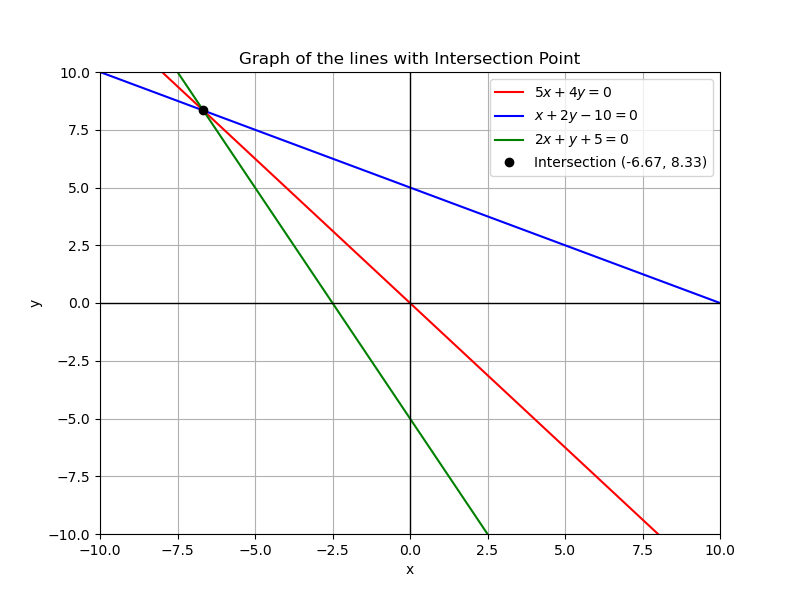
\includegraphics[width=0.8\linewidth]{figs/01.png}
   \caption{Plot of the three lines}
   \label{Plot_1}
\end{figure}
\end{frame}

 % --------- CODE APPENDIX ---------
\section*{Appendix: Code}

% C program
\begin{frame}[fragile]{File: points.c}
\begin{lstlisting}[language=C]
#include <stdio.h>

int main() {
  FILE *fp;

  // -------------------
  // Question 4.13.68
  // -------------------


  fp = fopen("points.dat", "w");
  fprintf(fp, "%d,%d,%d\n", 5, 4, 0);  // n1 c1
  fprintf(fp, "%d,%d,%d\n", 1, 2, 10);   // n2 c2
  fprintf(fp, "%d,%d,%d\n", 2, 1, -5); // n3 c3
  fclose(fp);
  return 0;
}
\end{lstlisting}
\end{frame}

% Python calling C
\begin{frame}[fragile]{File: call\_c.py}
\begin{lstlisting}[language=Python]
import subprocess

# Compile the C program
subprocess.run(["gcc", "points.c", "-o", "points"])

# Run the compiled C program
result = subprocess.run(["./points"], capture_output=True, text=True)

# Print the output from the C program
print(result.stdout)
\end{lstlisting}
\end{frame}

% Python plotting
\begin{frame}[fragile]{File: plot.py}
\begin{lstlisting}[language=Python]
import numpy as np
import matplotlib.pyplot as plt
from sympy import symbols, Eq, solve

# Define the symbols
x, y = symbols('x y')

# Define the equations
eq1 = Eq(5*x + 4*y, 0)          # 5x + 4y = 0
eq2 = Eq(x + 2*y - 10, 0)       # x + 2y - 10 = 0

# Solve the system of two equations
solution = solve((eq1, eq2), (x, y))

# Extract the intersection point
intersection_x = solution[x]
intersection_y = solution[y]

# Define the lines
def line1(x):
    return (-5*x) / 4

def line2(x):
    return (10 - x) / 2

def line3(x):
    return (-2*x - 5)

# Generate x values
x_vals = np.linspace(-10, 10, 400)
\end{lstlisting}
\end{frame}

% Python plotting
\begin{frame}[fragile]{File: plot.py}
\begin{lstlisting}[language=Python]
# Plot the lines
plt.figure(figsize=(8, 6))
plt.plot(x_vals, line1(x_vals), label=r'$5x + 4y = 0$', color='r')
plt.plot(x_vals, line2(x_vals), label=r'$x + 2y - 10 = 0$', color='b')
plt.plot(x_vals, line3(x_vals), label=r'$2x + y + 5 = 0$', color='g')

# Mark the point of intersection
plt.plot(intersection_x, intersection_y, 'ko', label=f'Intersection ({intersection_x:.2f}, {intersection_y:.2f})')

# Set plot limits and labels
plt.xlim(-10, 10)
plt.ylim(-10, 10)
plt.axhline(0, color='black',linewidth=1)
plt.axvline(0, color='black',linewidth=1)
plt.grid(True)

# Labeling
plt.title('Graph of the lines with Intersection Point')
plt.xlabel('x')
plt.ylabel('y')

# Adding a legend
plt.legend()

# Show plot
plt.show()
\end{lstlisting}
\end{frame}

\end{document}
